%
% File acl2014.tex
%
% Contact: koller@ling.uni-potsdam.de, yusuke@nii.ac.jp
%%
%% Based on the style files for ACL-2013, which were, in turn,
%% Based on the style files for ACL-2012, which were, in turn,
%% based on the style files for ACL-2011, which were, in turn, 
%% based on the style files for ACL-2010, which were, in turn, 
%% based on the style files for ACL-IJCNLP-2009, which were, in turn,
%% based on the style files for EACL-2009 and IJCNLP-2008...

%% Based on the style files for EACL 2006 by 
%%e.agirre@ehu.es or Sergi.Balari@uab.es
%% and that of ACL 08 by Joakim Nivre and Noah Smith

\documentclass[11pt]{article}
\usepackage{paper}
\usepackage{times}
\usepackage{algorithm}
\usepackage{algpseudocode}
\usepackage{multirow}
\usepackage{url}
\usepackage{latexsym}
\usepackage[utf8]{inputenc}
\usepackage{graphicx}
\usepackage{color}

%\setlength\titlebox{5cm}

% You can expand the titlebox if you need extra space
% to show all the authors. Please do not make the titlebox
% smaller than 5cm (the original size); we will check this
% in the camera-ready version and ask you to change it back.


\title{Comparación de Metaheurísticas y Algoritmos Poblacionales
       para Selección de Instancias}

\author{Formica, Gabriel\\
  Universidad Simón Bolívar\\
  Caracas, Venezuela\\
  {gabrielformica93@gmail.com} \\\And
  Ponte, José Antonio\\
  Universidad Simón Bolívar\\
  Caracas, Venezuela\\
  {pontezambrano@gmail.com} \\}

\date{}

\begin{document}
\maketitle

\begin{abstract}
  El problema de \textit{Selección de Instancias}  busca
  escoger un subconjunto de instancias de menor cardinalidad del conjunto original
  que mantenga la clasificación de las muestras a ser usadas como un conjunto
  de entrenamiento. En este articulo se considera la resolución de este problema mediante varios algoritmos metaheurísticos de trayectoria y poblacionales. Particularmente se consideran las técnicas Tabu, ILS, Memético y SGA. Se comparan estas implementaciones con un conjunto extenso de datos y se extraen conclusiones acerca de su desempeño en tiempo y calidad de solución.
\end{abstract}

\section{Introducción}
  En este trabajo se considera el problema de Selección de Instancias, como
  estrategia de reducción de datos para aplicación de procesos de KDD. Dado un conjunto de
  instancias de datos, el problema de 
  \textit{Selección de Instancias} (IS por sus siglas en inglés), busca
  escoger un subconjunto de instancias de menor cardinalidad que el conjunto original
  que mantenga o mejore la clasificación de las muestras a ser usadas como un conjunto
  de entrenamiento. 
  
  En el presente trabajo se implementan 2 Metaheurísticas de trayectorias 
  (ILS, Tabú) y 2 Metaheurísticas poblacionales (Algoritmo Memético y 
  SGA (Stationary Genetic Algorithm por sus siglas en inglés), 
  mostrando para cada una de ellas los resultados 
  y tiempos de corrida al aplicarlas sobre diferentes conjuntos de datos.

  Este trabajo se organiza en 6 secciones. Se comienza con una definición
  formal del problema, en donde se explica la terminología relevante a SI. 
  Posteriormente, se describe la representación de las soluciones, así 
  como también el proceso de generación de soluciones iniciales. Se continúa
  con los algoritmos y metaheurísticas usadas, mostrando el pseudocódigo de cada
  una de ellas. Seguido a esto, se describen cada uno de los conjuntos de datos usados
  en los experimentos. Finalmente, se presentan los resultados experimentales y se 
  concluye en base a dicho resultados.

\section{Definición del Problema}

Un conjunto de datos se define en función de un conjunto de clases $\Omega$ y
un conjunto de $n$ observaciones $T$. Un problema de SI se define entonces como dicho 
conjunto de instancias 
$T = \{t_{1}, t_{2},..., t_{n}\}$, donde una instancia (observación) $t_{i}$ es
una tupla $t_{i} = (v_{i,1}, v_{i,2},...,v_{i,m})$ de $m$ valores/mediciones
(un punto en un espacio m-dimensional). Además, cada instancia $t_{i}$
pertenece a una clase $w_{t_{i}}  \epsilon  \Omega$. 

La idea es seleccionar un subconjuto de menor cardinalidad 
$R \subseteq T$ tal que $R$ mantega o mejore la capacidad 
de representación del conjunto $T$.

\section{Descripción de la solución}

En esta sección se muestra al lector el proceso de construcción de una 
solución. Especificamente, se muestra cómo se representa una solución,
cómo se generan las soluciones iniciales, y finalmente, se incluye 
el pseudocódigo de la metaheurística implementada.

\subsection{Representación}

Sea un conjunto inicial $T$, una solución al problema de SI está
dado por un subconjuto de instancias $R$,
que puede ser fácilmente representado por una cadena de bits de 
tamaño $n = |T|$ donde cada bit tiene valor 1/0, indicando respectivamente,
la pertenencia o no de una instancia $t_{i} \epsilon T$ en la solución. 

\subsection{Generación de soluciones iniciales}

Siendo una representación una cadena de bits, para generar una solución
inicial seguimos una estrategia muy sencilla: cada bit tiene una probabilidad $\rho$
de estar en la solución. Si bien en la literatura, lo común es
que $\rho$ sea igual a $0.5$, de manera de comenzar con un solución
de $50\%$, en nuestro caso hemos hecho varias ``corridas'' con distintos valores
de $\rho$, generando soluciones iniciales de distintos tamaños, de manera de poder
evaluar el impacto de cada una de estas reducciones.

\section{Función de evaluación}
En (Cano et. al 2003) se describe una función de evaluación que considera la tasa de instancias clasificadas correctamente tomando en cuenta el conjunto reducido como conjunto de entrenamiento y una tasa de reducción del conjunto original. Se hace uso de una constante $\alpha$ donde $\alpha \in [0,1]$ para darle ponderación a ambos parámetros. La fórmula usada para medir la calidad de una solución es:

~\

\begin{center}
    {\fontsize{10}{10}\selectfont
    $ evaluar(R) = \alpha \times tasa\_clas + (1 - \alpha) \times porcen\_redc $
    }
\end{center}

~\

El objetivo de un algoritmo es maximizar esta función, entonces si $evaluar(A) < evaluar(B)$, se tiene que $B$ es mejor solución que $A$. Para los experimentos se usó la tasa sugerida por (Cano et. al 2003) de $\alpha = 0.5$ dándole la misma ponderación a $tasa\_clas$ y a $porcen\_redc$.

\section{Algoritmos}

    Para los algoritmos basados en poblaciones, se utilizó como operador de mutación el cruce en un punto (\emph{one-point crossover}), mientras que para la selección se usó la técnica de torneo (\emph{tourney selection}) con un torneo de tamaño 3.

    \subsection{Tabú}
    Tabú mantiene una \emph{lista tabú} en la cual mantiene un historial de soluciones candidatas recientemente consideras 
    y rechaza retornar dichos candidatos hasta que estén lo suficientemente en el pasado. De esta manera,


    {\fontsize{9}{12}\selectfont
    \begin{algorithmic}
        \Function{Tabú}{$T: Problema, S: Solution, l: Entero, N: Entero$}
            \State $S$ \Comment{Solución candidata}
            \State $N$ \Comment{Numero de tweaks a aplicar}
            \State $l$ \Comment{Largo máximo de la lista tabu}
            \State $Mejor \gets S$ 
            \State $Tabu \gets {}$  \Comment{Lista tabu inicialmente vacía}
            \State $Tabu \gets S \cup Tabu$ 
            \While{$\lnot condicionDeParada$}
                \If{\Call{length}{$Tabu$} $>$ $l$}
                    \State \Call{removeOldestElement}{$Tabu$}
                \EndIf
                \State $R \gets \Call{tweak}{S}$
                \For{$N - 1 \ veces$}
                \State $S' \gets \Call{copy}{S}$
                \State $W \gets \Call{tweak}{S'}$
                \If{W no peternece a Tabu Y ($\Call{quality}{W} > \Call{quality}{R}$
                    O R pertenece a Tabu)}
                    \State $R \gets W$
                \EndIf
            \EndFor
            \If{R no peternece a Tabu Y ($\Call{quality}{R} > \Call{quality}{S}$}
                \State $S \gets R$
                \State $Tabu \gets R \cup Tabu$ 
            \EndIf
            \If{$\Call{quality}{S} > \Call{quality}{Mejor}$}
                \State $Mejor \gets S$
            \EndIf
            \EndWhile
            \State return $Mejor$
        \EndFunction
    \end{algorithmic}
    }

    ~\ 

    Como condición de parada se establece que el mínimo de calidad de una solución sea $0.95$ y una cantidad determinada de iteraciones en las cuales la solución no cambie.

    \subsection{ILS}
    ILS es basicamente una versión mejorada de Hill-Climbing con reinicios aleatorios. A continuación, se presenta al lector el pseudo-código:


    {\fontsize{9}{12}\selectfont
    \begin{algorithmic}
        \Function{ILS}{$T: Problema, S: Solution,  t: Entero$}
            \State $t$ \Comment{Tiempo para reinicio}
            \State $S$ \Comment{Solución inicial}
            \State $Mejor \gets S$
            \While{$\lnot condicionDeParada$}
                \State $time \gets numero aleatorio en base a t$

                \While{$\lnot condicionDeParadaInterna$}
                    \State $S' \gets \Call{copy}{S}$
                    \State $R \gets \Call{tweak}{S'}$
                    \If{$\Call{quality}{R} > \Call{quality}{S}$}
                        \State $S \gets R$
                    \EndIf
                \EndWhile
            \If{$\Call{quality}{S} > \Call{quality}{Mejor}$}
                \State $Mejor \gets S$
            \EndIf
            \State $S \gets \Call{perturb}{S}$
            \EndWhile
            \State return $Mejor$
        \EndFunction
    \end{algorithmic}
    }

    ~\ 

    Como condición de parada se establece que el mínimo de calidad de una solución sea $0.95$ y una cantidad determinada de iteraciones en las cuales la solución no cambie.


    \subsection{Algoritmo poblacional híbrido (memético)}
    Para la busqueda poblacional híbrida se considera una combinación de la noción de población y mutación con la búsqueda local clásica.

    {\fontsize{9}{12}\selectfont
    \begin{algorithmic}
        \Function{Híbrido}{$T: Problema$}
            \State $Mejor \gets \Call{solucionAleatoria}$
            \State $P \gets \Call{poblacionAleatoria}$
            \While{$\lnot condicionDeParada$}
                \For{Cada $P_i$ en $P$}
                  \State $P_i \gets \Call{busquedaLocal}{T}$
                    \If{\Call{calidad}{$P_i$} $>$ \Call{calidad}{$Mejor$}}
                        \State $Mejor \gets P_i$
                    \EndIf
                \EndFor
            \State $P \gets \Call{reproducir}{P}$
            \EndWhile
            \State return $Mejor$
        \EndFunction
    \end{algorithmic}
    }

    ~\ 

    Como condición de parada se establece que el mínimo de calidad de una solución sea $0.95$ y una cantidad determinada de iteraciones en las cuales la solución no cambie. Adicionalmente, siempre se favorece la descendencia al reproducir la población.



    \subsection{SGA}
    Para el SGA se considera utiliza un criterio de selección elitista, es decir, los hijos sólo reemplazan a los padres si son mejores. \\

    {\fontsize{10}{12}\selectfont
    \begin{algorithmic}
        \Function{SGA}{$T: Problema$}
            \State $P \gets \Call{poblacionAleatoria}$
            \State $Mejor \gets $ mejor individuo en P
            \While{$\lnot condicionDeParada$}
                \State $P_1 \gets $ Seleccion de indv. de P  
                \State $P_2 \gets $ Seleccion de indv. de P 
                \State $c_1,c_2 \gets $ recombinar $P_1 y P_2$
                \State Mutar $c_1$ y $c_2$ 
                \If{$c_1$ y $c_2$ son mejores que $P_1$ y $P_2$}
                    \State Reemplazar
                \EndIf
                \State $Mejor' \gets $ mejor individuo en P 
                \If{$Mejor'$ $>$ $Mejor$}
                    \State $Mejor \gets Mejor'$
                \EndIf
            \EndWhile
            \State return $Mejor$
        \EndFunction
    \end{algorithmic}
    }

    ~\ 

    Como condición de parada se establece que el mínimo de calidad de una solución sea $0.95$ y una cantidad determinada de iteraciones en las cuales la solución no cambie.

\subsection{1NN}
    Para el cálculo de la calidad de una solución, se hace uso del clasificador $1NN$ que clasifica un conjunto usando un conjunto definido como entrenamiento. Sobre los resultados obtenidos de $1NN$ se corre una función de evaluación que asinga un valor a la solución. \\

    {\fontsize{10}{10}\selectfont
    \begin{algorithmic}
        \Function{Calidad}{$S: Solucion$, $T: Problema$}
            \State $Problema$  $entrenamiento$
            \State $Problema$  $resultado$
            \State $resultado \gets \Call{1NN}{entrenamiento, T}$
            \State $retorna$ $eval(resultado)$
        \EndFunction
    \end{algorithmic}
    }


\subsection{Operador}

Un operador de vencidad es una función que recibe una solución $S$,
retorna una solución $S'$,  \emph{Operador} : $S$ -> $S'$, donde $S'$ es una solución \emph{un poco} distinta
a $S$, y que tiende a ser mejor.

Se implementó un operador de vencidad, el cual llamamos \emph{weightedRandomPlus}.
Este operador tiene parametrizado una \emph{probabilidad de reducción} y
un \emph{porcentaje de operación}. 

El \emph{porcentaje de operación} (que llamaremos $Po$ es básicamente
indica sobre cuantos bits de la solución se operarán. Así si $Po = 10 \%$,
y el \emph{data set} es de tamaño $1000$, entonces se operará sobre
$100$ bits de la solución.

Una vez que se sabe la cantidad de bits a operar $c = Po * 1000 = 100$,
la \emph{probabilidad de reducción} (que llamaremos $Pr$)
decidirá qué hacer con un proximo bit.
Si $Pr = 60 \% = 0.6$, y un número escogido aleatoremente $0 \le n_{r} \le 1.0$
es también $n_{r} \le Pr$, se escogerá un bit aleatoremanete y que esté
\emph{prendido}, con el fin de apagarlo. En caso contrario que $n_{r} > Pr$,
se escogerá aleatoreamente un bit \emph{apagdo} para prenderlo. A continuación
se presenta el pseudo-código del operador. \\


    {\fontsize{10}{10}\selectfont
    \begin{algorithmic}
        \Function{weightedRandomPlus}{$S: Solucion$, $sz: Entero$, 
                                      $Pr: Entero$, $Po: Entero$}
        \State $c \gets Po * sz$  \Comment{sz es el tamaño de dataset} 
          \For{$i \gets 1 \textbf{ to } c$}
                \State $rand \gets getRand()$    \Comment{Entre 0 y 1} 
                \If{$rand < Pr$}
                \State $\Call{apagarBitPrendido}$ 
                \Else
                \State $\Call{prenderBitApagado}$ 
                \EndIf
            \EndFor
            \State return $S$
        \EndFunction
    \end{algorithmic}
    }

    ~\ 

  Recordando que \emph{apagarBitPrendido} escoge un aleatoreamente un bit prendido,
  y  que \emph{prenderBitApagado} escoge un aleatoreamente un bit apagado.

\section{Evaluación Experimental}

La tarea principal de la evaluación experimental en este trabajo es evaluar el desempeño de distintas metaheurísticas sobre varios conjuntos de datos. Dicho desempeño se mide mediante tres indicadores: 
\begin{itemize}
\item Porcentaje reducción 
    Porcentaje al cual se reduce el conjunto de entrenamiento
\item Tasa de errores de validación
    Tasa de errores de clasificación del conjunto de validación usando el conjunto de entrenamiento reducido.
\item tiempo de ejecución
    Tiempo de ejecución de una corrida de la metaheurística
\end{itemize}


\subsection{Conjuntos de datos}
Los conjuntos de datos se escogieron intentando alcanzar un balance entre tener conjuntos similares entre sí en función de número de instancias y número de atributos, y conjuntos de datos que fueran diversos entre sí, tratando de abarcar el máximo espacio posible del universo de conjuntos de datos.

Los datos son obtenidos de \emph{KEEL Data-Mining Software Tool}. En la siguientes tablas se muestran los conjuntos de datos considerados pequeños, medianos y grandes respectivamente.

\begin{table}[h]
\begin{tabular}{ |l|l|l|l|l| }
    \hline
    Caso    & Instancias & Atributos & Clases \\ \hline
    bupa & 345  & 6 &  2 \\ \hline
    ecoli & 336 & 7 & 8 \\ \hline
    glass & 214 & 9 & 10 \\ \hline
    haberman & 306 & 3 & 2 \\ \hline
    hayes-roth & 160 & 4 & 3 \\ \hline
    ionosphere & 351 & 33 & 2 \\ \hline
    iris & 150 & 4 & 5 \\ \hline
    monk-2 & 432 & 6 & 2 \\ \hline
    newthyroid & 215  & 5 & 3 \\ \hline
    saheart & 462 & 9 & 2 \\ \hline
    sonar & 208 & 60 & 2 \\ \hline
    wine & 178 & 13 & 3 \\ \hline
\end{tabular}
\caption{Conjuntos de datos pequeños}
\label{tabla:1}
\end{table}

\begin{table}[h]
\begin{tabular}{ |l|l|l|l|l| }
    \hline
    Caso    & Instancias & Atributos & Clases \\ \hline
    balance & 625  & 4 &  3 \\ \hline
    pima & 768  & 8 &  2 \\ \hline
    tic-tac-toe & 958  & 9 &  2 \\ \hline
    vehicle & 846  & 18 &  4 \\ \hline
\end{tabular}
\caption{Conjuntos de datos medianos}
\label{tabla:1}
\end{table}

\begin{table}[h]
\begin{tabular}{ |l|l|l|l|l| }
    \hline
    Caso    & Instancias & Atributos & Clases \\ \hline
    banana & 5300  & 2 &  2 \\ \hline
    abalone & 4174  & 8 &  28 \\ \hline
\end{tabular}
\caption{Conjuntos de datos grandes}
\label{tabla:1}
\end{table}

\subsection{Preparación de datos}

Cada experimento se ejecuta particionando el conjunto de datos en dos partes: entrenamiento y validación. La manera de hacer esto es que cada instancia tiene 90\% de probabilidad de estar en entrenamiento y 10\% de estar en validación. Para garantizar que no exista un sesgo en la escogencia de esta partición, se usa la técnica de validación cruzada en 10 grupos. Esto consiste en dividir el conjunto de datos D en 10 partes iguales $D_1, D_2, ..., D_{10}$. En función de estas particiones, se definen los pares $(D \setminus D_i, D_i)$. Cada metaheurística es evaluada usando estos pares y sobre cada par haciendo 5 corridas distintas.


\subsection{Parámetros}

Cada metaheurística se entonó hasta encontrar los parámetros que mejoraban el desempeño de la misma.

\begin{table}[h]
\scalebox{1}{
\begin{tabular}{ |l|l|l|l|l| }
    \hline
    Parámetro & ILS & Tabu & Hibrído & SGA  \\ \hline
    Iter. totales & 1000 & 1000 & 50 & 1000 \\ \hline
    Iter. locales & 100 & 100     & 10  & 100 \\ \hline
    Iter. sin cambio & 20 & 50     & 5  & 50 \\ \hline
    Tamaño de lista & - & 10    & -  & - \\ \hline
    \# de Tweaks & - & 5     & -  & - \\ \hline
    Población & - & -     & 20  & 30 \\ \hline
\end{tabular}
}
\caption{Parámetros usados en metaheurísticas}
\label{tabla:2}
\end{table}

\subsection{Ejecuciones}
Los experimentos se corrieron sobre computadores de procesador Intel(R) Core(TM) i7-3770 CPU @ 3.40GHz, con 8 GB de RAM sobre un sistema Debian Linux.

\subsection{Resultados}

\begin{table}[h]
\scalebox{0.6}{
\begin{tabular}{ |l|l|l|l|l|l| }
    \hline
        \multicolumn{6}{ |c| }{Casos de prueba grandes} \\
    \hline
    Caso & Heuristica & Err val & Tam Reduc & Error & Tiempo \\ \hline
    \multirow{4}{*}{Banana} & Tabu     & \bf{13.28302}   & 3.937526     &  \bf{70.4}   & 53.3222 \\
                            & ILS      & 13.31699   & \bf{1.305241}     &  70.58  & 591.7742 \\
                            & Memetico & 14.02265   & 1.47631      &  74.32  & 172.797 \\
                            & SGA      & 14.49056   & 2.111949     &  76.8   & \bf{35.232}\\ \hline
\end{tabular}
}
\end{table}

\begin{table}[h]
\scalebox{0.6}{
\begin{tabular}{ |l|l|l|l|l|l| }
    \hline
        \multicolumn{6}{ |c| }{Casos de prueba pequeños} \\
    \hline
    Caso & Heuristica & Err val & Tam Reduc & Error & Tiempo \\ \hline
    \multirow{4}{*}{Bupa} & Tabu     & 35.13766         & 0.97264      &  12.12          & 0.5884 \\
                             & ILS      & \bf{31.28007} & \bf{0.889045}     &  \bf{10.8} & 4.1052 \\
                             & Memetico & 33.99377      & 0.92767      &  11.72          & 1.7144 \\
                             & SGA      & 39.48908      & 1.320954     &  13.62          & \bf{0.3142}\\ \hline
    \multirow{4}{*}{Ecoli}   & Tabu     & 30.85025      & \bf{2.55893}      &  10.38  & 0.6244 \\
                             & ILS      & \bf{26.52584} & 4.028173     &  \bf{8.92}   & 7.0984 \\
                             & Memetico & 29.12677      & 3.643914     &  9.8    & 1.9566 \\
                             & SGA      & 28.8253       & 5.3836       &  9.7    & \bf{0.3122}\\ \hline
    \multirow{4}{*}{Glass}   & Tabu     & 40.26272   & \bf{4.080946}     &  8.66   & 0.3336 \\
                             & ILS      & \bf{37.98743}   & 4.327704     &  \bf{8.22}   & 3.7046 \\
                             & Memetico & 38.22237   & 4.659532     &  8.24   & 1.2344 \\
                             & SGA      & 38.49303   & 8.02254      &  8.3    & \bf{0.18}\\ \hline
    \multirow{4}{*}{Haberman}   & Tabu     & 25.86667   & 0.994915        &  7.9    & 0.429 \\
                                & ILS      & \bf{25.80216}   & 0.893281   &  \bf{7.88}   & 2.9763 \\
                                & Memetico & 26.38925   & 0.944243        &  8.06   & 1.0734 \\
                                & SGA      & 26.41724   & \bf{0.58108}    &  8.08   & \bf{0.1846}\\ \hline
    \multirow{4}{*}{Ionosphere}   & Tabu     & 16.07302   & 2.272815     &  5.64   & 1.5468 \\
                                  & ILS      & \bf{13.40159}   & 2.279123     &  \bf{4.7}    & 15.304 \\
                                  & Memetico & 15.16667   & \bf{2.044946}     &  5.32   & 5.7892 \\
                                  & SGA      & 17.27461   & 4.868776     &  6.06   & \bf{1.0562}\\ \hline
    \multirow{4}{*}{Iris}   & Tabu     & \bf{5.733331}   & 3.970368     &  \bf{0.86}   & 0.0348 \\
                            & ILS      & \bf{5.73333}    & \bf{3.659257}     &  \bf{0.86}   & \bf{0.0152} \\
                            & Memetico & 6.39999         & 3.99999      &  0.96   & 0.1462 \\
                            & SGA      & 5.86666         & 4.992591     &  0.88   & 0.452\\ \hline
    \multirow{4}{*}{Monk-2}   & Tabu     & 19.3827    & 1.419281     &  8.32   & 0.8218 \\
                              & ILS      & \bf{11.77317}   & \bf{1.389261}     &  \bf{5.1}    & 7.9858 \\
                              & Memetico & 15.78001   & 1.394267     &  6.82   & 2.5364 \\
                              & SGA      & 18.3673    & 4.473317     &  7.96   & \bf{0.4278}\\ \hline
    \multirow{4}{*}{Newthyroid}   & Tabu     & 11.64502   & 2.53245      &  2.5    & 0.2808 \\
                                  & ILS      & \bf{9.748918}   & \bf{2.191604}     &  \bf{2.1}    & 2.1954 \\
                                  & Memetico & 10.49351   & 2.811653     &  2.6    & 0.7974 \\
                                  & SGA      & 11.70563   & 5.405375     &  2.52   & \bf{0.1154}\\ \hline
    \multirow{4}{*}{Saheart}  & Tabu     & 33.50879   & 0.683068     &  15.48  & 1.0738 \\
                              & ILS      & \bf{32.72987}   & 0.586793     &  \bf{15.12}  & 5.7216 \\
                              & Memetico & 33.91212   & 0.69262      &  15.66  & 2.9838 \\
                              & SGA      & 34.41073   & \bf{0.471327}     &  15.9   & \bf{0.6406}\\ \hline
    \multirow{4}{*}{Sonar}  & Tabu     & 39.0095    & 1.891115     &  8.1    & 1.067 \\
                            & ILS      & 33.8666    & \bf{1.698715}     &  7.04   & 8.053 \\
                            & Memetico & \bf{32.32379}   & 2.275174     &  \bf{6.72}   & 4.1412 \\
                            & SGA      & 35.09998   & 6.571566     &  7.3    & \bf{0.719}\\ \hline
    \multirow{4}{*}{Wine} & Tabu     & \bf{28.10458}   &  2.32212     &  \bf{5.0}      & 0.3314 \\
                          & ILS      & 28.9085    &  2.322049    &  5.14   & 2.5746 \\
                          & Memetico & 28.69935   &  \bf{2.11015}     &  5.1    & 0.9834 \\
                          & SGA      & 30.24836   &  3.258773    &  5.38   & \bf{0.1628}\\ \hline
    \multirow{4}{*}{Saheart}  & Tabu     & 33.50879   & 0.683068     &  15.48  & 1.0738 \\
                              & ILS      & \bf{32.72987}   & 0.586793     &  \bf{15.12}  & 5.7216 \\
                              & Memetico & 33.91212   & 0.69262      &  15.66  & 2.9838 \\
                              & SGA      & 34.41073   & \bf{0.471327}     &  15.9   & \bf{0.6406}\\ \hline
\end{tabular}
}
\end{table}

\newpage
\vfill

\begin{table}[h]
\scalebox{0.6}{
\begin{tabular}{ |l|l|l|l|l|l| }
    \hline
        \multicolumn{6}{ |c| }{Casos de prueba medianos} \\
    \hline
    Caso & Heuristica & Err val & Tam Reduc & Error & Tiempo \\ \hline
    \multirow{4}{*}{Australian}   & Tabu     & 33.3913     & 0.42512  & 23.04 & 2.6786 \\
                                  & ILS      & \bf{31.5072} & \bf{0.412238} & \bf{21.74} & 15.253 \\
                                  & Memetico & 33.42028   & \bf{0.412238} & 23.06 & 8.322 \\
                                  & SGA      & 37.2463    & 1.07246  & 25.7  & \bf{2.018}\\ \hline
    \multirow{4}{*}{Balance} & Tabu     & 16.2951    &  0.5155      &  10.18  & 1.3566 \\
                             & ILS      & \bf{12.8966}    &  \bf{0.444467}    &  \bf{8.06}   & 10.0512 \\
                             & Memetico & 14.2838    &  0.462071    &  8.92   & 4.0198 \\
                             & SGA      & 20.70254   &  2.179019    &  12.94  & \bf{0.7512}\\ \hline
    \multirow{4}{*}{Pima}   & Tabu     & 26.13381   & 0.355893     &  20.08  & \bf{2.2424} \\
                            & ILS      & \bf{25.74077}   & 0.32985      &  \bf{18.78}  & 12.0942 \\
                            & Memetico & 26.20867   & \bf{0.3240552}    &  20.14  & 6.8738 \\
                            & SGA      & 30.4033    & 0.8534       &  23.36  & 16198.0\\ \hline
    \multirow{4}{*}{Tic-Tac-Toe}   & Tabu     & 34.52851   & 0.4338048    &  33.08  & 3.063 \\
                                   & ILS      & \bf{33.0}         & 1.16216      &  \bf{31.62}  & 16.518 \\
                                   & Memetico & 34.09035   & 0.9440143    &  32.66  & 10.2386 \\
                                   & SGA      & 34.75614   & \bf{0.3804321}    &  33.3   & \bf{2.5356}\\ \hline
    \multirow{4}{*}{Vehicle}  & Tabu     & 49.09916   & 3.123149     & 41.54   & 41.54 \\
                              & ILS      & \bf{46.66246}   & 3.070576     & \bf{39.48}   & 56.56 \\
                              & Memetico & 47.49272   & \bf{3.054687}     & 40.18   & 18.8208 \\
                              & SGA      & 45.90784   & 4.85396      & 38.84   & \bf{3.509}\\ \hline
    \multirow{4}{*}{WDBC} & Tabu     & 8.681703   & 0.7069326    & 4.94    & 2.3308 \\
                          & ILS      & 9.489349   & \bf{0.601433}     & 5.4     & \bf{0.5102} \\
                          & Memetico & \bf{8.365288}   & 0.7850499    & \bf{4.76}    & 7.4894 \\
                          & SGA      & 9.243108   & 1.241914     & 5.25    & 2.1942\\ \hline
\end{tabular}
}
\end{table}

\clearpage
\newpage

\begin{figure}[h!]
\begin{center}
  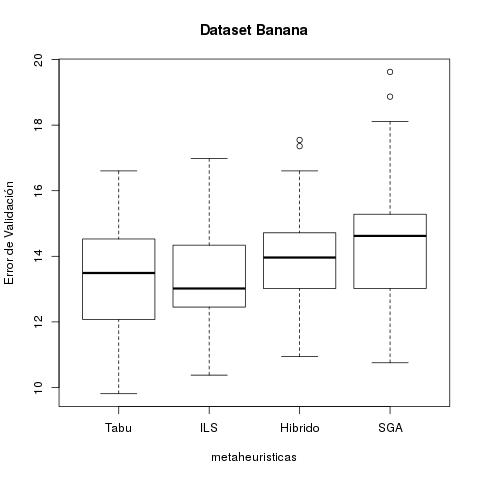
\includegraphics[scale=0.4]{banana_error_val.jpeg}~\\[1cm]
\end{center}
\end{figure}

\begin{figure}[h!]
\begin{center}
  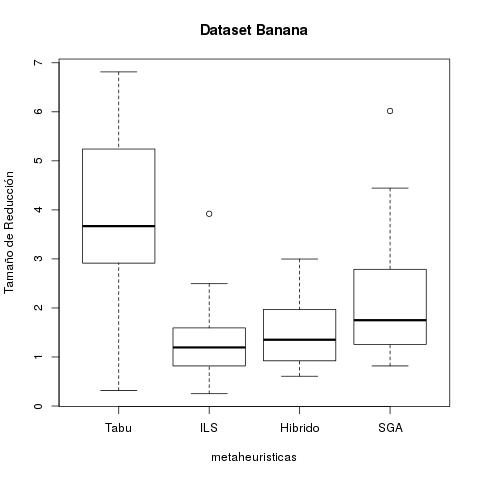
\includegraphics[scale=0.4]{banana_tam_reduc.jpeg}~\\[1cm]
\end{center}
\end{figure}

\begin{figure}[h!]
\begin{center}
  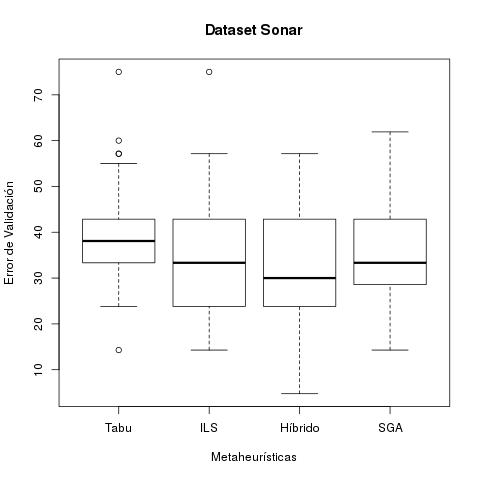
\includegraphics[scale=0.4]{sonar_err_val.jpeg}~\\[1cm]
\end{center}
\end{figure}

\begin{figure}[h!]
\begin{center}
  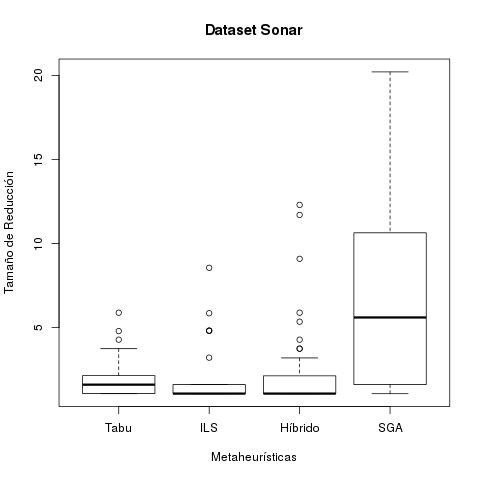
\includegraphics[scale=0.4]{sonar_tam_red.jpeg}~\\[1cm]
\end{center}
\end{figure}

\begin{figure}[h!]
\begin{center}
  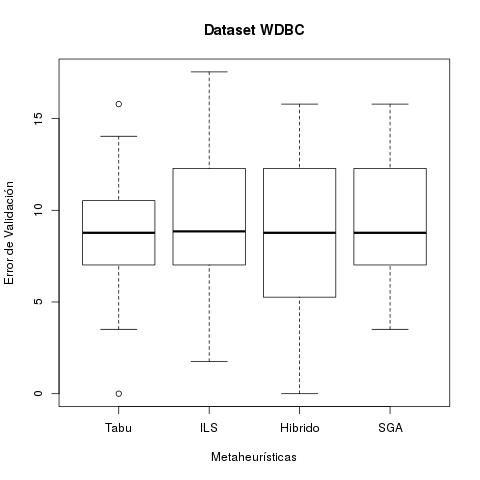
\includegraphics[scale=0.4]{wdbc_err_val.jpeg}~\\[1cm]
\end{center}
\end{figure}

\clearpage

\begin{figure}[h!]
\begin{center}
  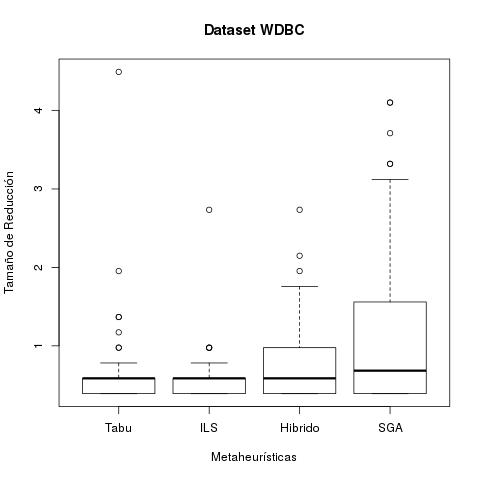
\includegraphics[scale=0.4]{wdbc_tam_red.jpeg}~\\[1cm]
\end{center}
\end{figure}


% \newpage
\section{Conclusiones y recomendaciones}

Las metaheurísticas lograron resolver en gran medida el problema propuesto. Considerando los porcentajes promedio de reducción y de errores de validación se observan resultados prometedores para los casos evaluados. El mayor espacio a mejora se encuentra en los errores de validación, para lo cual se debe considerar evaluar entonaciones adicionales sobre los operadores usados por las metaheurísticas.

Se hace evidente además que las metaheurísticas funcionan de una manera por casos, por lo cual los parámetros para un conjunto de datos no necesariamente son buenos para otro. Por lo cual se requiere un estudio más avanzado de cada uno de los conjuntos de datos que se quieran tratar.

En general, si se está buscando rapidez, las metaheurísticas de Tabu y SGA tienen un tiempo menor de corrida, sin embargo, para este trabajo se necesita mayor cuidado en la entonación de ésta última ya que fue común que sus resultados no fueran tan buenos como los de otros. Análogamente, la técnica con mejor desempeño en detrimento del tiempo fue el algoritmo memético.

% include your own bib file like this:
%\bibliographystyle{acl}
%\bibliography{acl2014}

\begin{thebibliography}{}

\bibitem[\protect\citename{Cano et al}2003]{Cano:03}
José Ramón Cano, Francisco Herrera, and Manuel Lozano.
\newblock 2003.
\newblock {\em Using evo-
lutionary algorithms as instance selection for data reduction in kdd: an
experimental study.}.
\newblock Evolutionary Computation, IEEE Transactions.

\bibitem[\protect\citename{Toussaint}200]{Toussaint:02}
Godfried Toussaing.
\newblock 2002.
\newblock {\em Proximity Graphs for Nearest Neighbor Decision Problem}.
\newblock School of computer science. McGill University

\bibitem[\protect\citename{Essentials of Metaheuristics}2013]{Sean:01}
Luke, Sean
\newblock 2013
\newblock {\em Essentials Of Metaheuristics}. 
\end{thebibliography}

\end{document}
